\documentclass[a6paper,10pt]{article}
%\usepackage[T1]{fontenc}
\usepackage[british]{babel}
\usepackage[utf8]{inputenc}
\usepackage{float, graphicx,amsmath,amsfonts,cite,enumerate,tabularx}
\usepackage[final]{pdfpages}
\usepackage{wrapfig}
\usepackage[margin=0.3in]{geometry}
\usepackage{sidspaltHack}

\newcommand{\mel}[1]{\small\textbf{\textit{mel. #1 \\}}}


\setlength{\oddsidemargin}{-0.37in}
\setlength{\textwidth}{215pt}

\pagestyle{empty}

\begin{document}
\nysida{15}{}
\noindent
\huge{$\Sigma\sigma$ Visor vi minns}
\vspace{10pt}

\noindent
\small
På denna sida börjar sångbokens nyaste kapitel: Sigma! Vårt mål med att införa ett kapitel som detta är att försöka \textit{summera} det gångna året på Fysiksektionen som det sett ut, eller snarare hörts ut, under gasquer, banquetter, spex eller övriga tillställningar. 

Häri finner du ett urval av de sångbladstexter, gyckel och spextexter som vi märkt varit uppskattade och lyckats fånga upp. Detta innebär förstås att vi missat flertalet fantastiska alster, men vi hoppas att det vi fått med är ett tillräckligt bra tidsdokument av läsåret 18/19. 

För er som var där väcker det (förhoppningsvis) roliga minnen och för er som inte var det kanske det ger ett smakprov på hur det kan låta på en gasque. Det som inte skrivs i bläck försvinner i tidens töcken, och vi kunde inte låta världen glömma vare sig Tentapokalyps, Mars \& Mello eller Skandal!. 

Vill du få med ett gyckel/en sångtext/en fin visa till nästa års summering? Tveka inte då att tipsa oss och/eller 2020 års sångboksansvariga och framför din åsikt! Många av texterna du finner här är med tack vare ivriga tips och hjälp från andra fysiker (ingen nämnd, ingen glömd). 

Mycket nöje i resan genom historien! 
\begin{flushright}
\textit{Adam Erlandsson och Filip af Malmborg, Förarlös \\Sångboksansvariga 2019}
\end{flushright}
\nysida{15}{19.1}
\setlength{\oddsidemargin}{-0.47in}

\begin{center}
\huge \textit{2018/2019}
\end{center}
\begin{center}
\LARGE Mottagningen \\
\end{center}
\begin{center}
\Large $\sigma19.1$. Balladen om enhörningen och nubben hon tog \\
\mel{Balladen om Theobald Thor} 
\end{center}
\small Det var en enhörning som var tuff\\
Och åt ett mål av nått regnbågsfluff\\
För att åt sittningen ge en puff\\
så tog hon till nubbe en sup
\vspace{5pt}\\
Och det var en stor sup,\\
mer än hon borde till lunch\\
Den var nog åt en hop,\\
ja en tre-fyra stop\\
Och sedan en lika stor punsch punsch punsch,\\
punscheli-punsch punsch punsch.
\vspace{5pt}\\
Allt blev svart tills idag blev igår\\
Hon vaknade fastspänd på en bår\\
Njurar fanns två men bland hennes hår\\
Av hornet fanns inte ett spår
\vspace{5pt}\\
Utom ett stort sår\\
Hennes horn var malet till krunch\\
Att på pinsam farsot,\\
impotens råda bot,\\
Efter att ha blandats i punsch...
\newpage
\setlength{\oddsidemargin}{-0.37in}
\noindent
Vår enhörning blev nykterist\\
Att dricka alkfritt gick väl visst\\
Men vad till avec som inte är trist\\
För att inte i pannan få hål?
\vspace{5pt}\\
Du tar en stor skål\\
Släng ut gårdagens brunch\\
Rör arom, sockerlag\\
Och kameliablad\\
Voila! Där har du din punsch!

\begin{flushright}
\textit{Anton Åkesson F-14, Stuggasquen 2018}
\end{flushright}

\nysida{15}{19.2}
\setlength{\oddsidemargin}{-0.47in}


\begin{center}
\Large $\sigma19.2$. nØllan mer\\ 
\mel{Better Now}
\end{center}\small$\|$: Jag ser ni tror ni ej är nØllan mer, nØllan mer!\\
Och att ni ganska snart blir fysiker, fysiker!\\
Nej, ingen aning vad som väntar er, väntar er!\\
När ni börjar KTH, när ni börjar KTH :$\|$
\vspace{5pt}\\
Dagen när ni dykte upp i Sing-Sing.\\
Foto, kåsa, fotleken i stor ring.\\
Arvingarna blastas dag ut, dag in.\\
Lära sig att gyckla, sjunga viking.
\vspace{5pt}\\
Infopass på dagen, hur ser vår framtid ut?\\
Övningsgasque med tempon och de tog aldrig slut.\\
Gyckel om ett Föhseri, skall kasta dem ut.\\
Buren ut som sopsäckar och gycklet tog slut.
\vspace{5pt}\\
Och ni åkte, åkte i väg,\\
ut i staden och till Alvik, ut här,\\
upp på morgonen och inte alls seg.\\
Men det här är bara ert första steg!
\vspace{5pt}\\
$\|$: Jag ser ni tror ni ej är nØllan mer, nØllan mer!\\
Och att ni ganska snart blir fysiker, fysiker!\\
Nej, ingen aning vad som väntar er, väntar er!\\
När ni börjar KTH, när ni börjar KTH :$\|$
\begin{flushright}
\textit{Yashar Honarmandi, F-17\\ Stuggasquen 2018}
\end{flushright}


\nysida{15}{19.3}
\setlength{\oddsidemargin}{-0.37in}
\vspace{35pt}

\begin{center}
\Large $\sigma19.3$. Julius Caesar \\ 
\mel{Jag vill vara din, Margareta}
\end{center}
\small Jag må vara din kalkylator, \\
men jag vet att du är Roms diktator. \\
Står vid stadens port, \\
vill ha dig hos mig fort, \\
förtrollad av din klinga!
\vspace{5pt} \\
Blickarna de känns, åh så heta! \\
känner du som jag, Julius Caesar? \\
Blickarna Du gav, gav Du dom som svar till en sej?
\vspace{5pt} \\
Dina lår, tar jag med, till Grekistan. \\
Sådant hår, fina tår, ger mig sår. \\
Kan inte hjälpa att jag vill vara dig när
\vspace{5pt} \\
Står vid stadens port, \\ 
vill ha dig hos mig fort\\
förtrollad av din klinga!  	
\vspace{5pt}\\
Blickarna de känns, åh så heta!\\
Känner du som jag, Julius Caesar?\\
Blickarna Du gav, gav Du dom som svar till en sej?

\begin{flushright}
\textit{nØllespexet 2018: Det Rätvinkliga Triangeldramat}
\end{flushright}

\nysida{15}{19.4}
\setlength{\oddsidemargin}{-0.47in}

\begin{center}
\LARGE Tentagasquer \\
\end{center}
\begin{center}
\Large $\sigma19.4$. Ingen vet ju vad jag gör\\ 
\mel{Ingen vill veta var du köpt din tröja}
\end{center} \small Tentan börjar 8, men jag brukar vara sen.\\
Sprang vilse i skogen innan modfysen\\
Går man via körsbärsvägen kan man spara nån minut\\
Men då får man räkna med att springa på Henelius   
\vspace{5pt} \\
På KTH vet jag att juni kan bli svår\\
Minst 45 hp för att få sitt CSN.\\ 
Men alla verkar nöjda och tentan är rättvis. \\ 
Nej, Clausius-Clapeyron skulle man kunna dess bevis?! För...
\vspace{5pt}\\
Inte vet jag vad jag gör, känner mig som en impostör.\\
Och min bordsgranne han andas väldigt högt.\\
Fast än jag gjort allt som man ska,\\
jag har pluggat på juldagen.\\
och jag har färgkodat varenda kapitel i Beta.
\vspace{5pt}\\
Nästa lördag kanske jag ska åka på släktträff.\\ 
Brukar börja bra, men slutar ofta med ett bråk.\\   
ingen av dem har 300 hp från KTH.\\         
Men de envisas med, att de visst förstår sig på mig, men...
\vspace{5pt}\\
Ingen vet ju vad jag gör, vad fan är en ingenjör?\\   
Ingen vill veta vad jag har för tenta\\
och fast jag förklarat som man ska,\\
jag har visat min kursplan,\\
tror min mormor att jag ska bli broarkitekt
\newpage
\setlength{\oddsidemargin}{-0.37in}
\noindent
Nej, ingen fattar vad jag gör,\\
jag är ingen IT reparatör.\\
Du kan väl fixa ditt jävla wifi på egen hand.\\
Och fast jag förklarat som man ska,\\
får jag alltid samma svar:\\
Vad pluggar du? Fysik! åh men jag älskar star trek.   
\vspace{5pt}\\
Förra hösten  minns jag, den var faktiskt riktigt fin.\\
Bo varenda dag, vi hade reglerteknik i Q.\\
Varje tal på tentan hade 40 deluppgifter.\\
skippar a) till h), men på i) ska man transformera
\vspace{5pt}\\
Lalalalalalalalalalalalalaplace\\
Lalalalalalalalalalalalalaplace
\vspace{5pt}\\
Men ingen vet ju vad de gör, i arbetslivet utanför\\
ingen är fullärd när de börjar som konsult\\
Och fast du läst en kex modul, om etik eller miljöstrul\\
Så kommer inte du att minnas vad dem sa.\\
Och fast du lärt dig kurstyptal\\
och fast bevis är trivialt\\    
Så finns det ingen som bryr sig på ditt jobb.\\
men med examen i din hand, har du visat att du kan\\
till torsdag lära dig allt relevant.

\begin{flushright}
\textit{Ebba Ahlgren, F-15\\ Tentagasque 1: Tentapokalyps}
\end{flushright}

\nysida{15}{19.5}
\setlength{\oddsidemargin}{-0.47in}


\begin{center}
\Large $\sigma19.5$. Skyddsrumsboogie\\
\end{center}\small Jag bara undrar när det gäller\\
När på allvar sirenen går\\
Finns det då skyddsrumsplatser, eller\\
Råder det brist på dem i år?\\
Måste man stå i skyddsrumskö\\
Och bli nobbad? - Tack och adjö!\\
Är det bara jag som ännu saknar reservation\\
Eller är vi fler som sjunger så här i sorgsen ton?
\vspace{5pt}\\
Ska man ha på sig aftondräkten?\\
Kastar de ut en stackars narr?\\
Blir det skit i skyddsrumsfläkten\\
För man har med sig sin gitarr?
\vspace{5pt}\\
Kräver dom på legitimation i porten\\
Eller blir det biljettkontroll?\\
Jo, konstapeln jag har inget kort, men\\
Inte spelar väl det nån roll?\\
Men hans min är hård och stel\\
Aldrig i livet ett tjänstefel\\
Portarna stängs, och då börjar man inse ganska klart\\
Döden närmar sig utan pardon i otrolig fart
\vspace{5pt}\\
Ska man ha på sig aftondräkten… 
\vspace{5pt}\\
Ja, då går man väl på krogen\\
Och där sitter min polare Pär\\
Tjenare, grabben! Jasså, det gick åt skogen?\\
Joru, grabben! Samma här!\\
Det skall vi fira med buller och bång\\
Sekunderna går sin gilla gång\\
Medan jag själv snabbt dricker upp\\
krögarens dyraste sprit\\
Utan en tanke på bakfylla eller kredit
\newpage
\setlength{\oddsidemargin}{-0.37in}
\noindent
Här har ingen på sig aftondräkten,\\
här är ingen den andres narr\\
Här blir det inte skit i fläkten\\
för man har med sig sin gitarr
\vspace{5pt}\\
Den som är ensam om ett skyddsrum,\\
måste väl ha privata skäl?\\
Vill han ensam överleva,\\
utan vänner som tar farväl?\\
Kanske han under jorden hör\\
Oss som sjunger här ovanför\\
Vila vid denna källa, hej, Samborombon!\\
Var skall man få sig en tom skyddsrumsplats ifrån?
\vspace{5pt}\\
Ska man ha på sig aftondräkten… 


\begin{flushright}
\textit{Text och musik av Cornelis Vreeswijk\\
Framförd av Filip af Malmborg, F-17\\ Tentagasque 1: Tentapokalyps}
\end{flushright}

\nysida{15}{19.6}
\setlength{\oddsidemargin}{-0.47in}

\begin{center}
\Large $\sigma19.6$. Triangel\\
\mel{Pippis sommarvissa}
\end{center}\small 
Idag så ska jag plugga, fastän jag inte vill.\\
Imorgon är ju tentan och hjärnan den står still.\\
Åh klockan är ju noll tre, och tentan åtta prick.\\
Åh fouriertransformer, det är en kul manick.\\
Det finns så många formler jag måste plugga in,\\
Och därför vill jag sova, jag fattar ingenting.
\begin{flushright}
\textit{Nicole Hedblom, F-17 \\ Tentagasque 2: Midsommar}
\end{flushright}


\begin{figure}[!h]
\centering
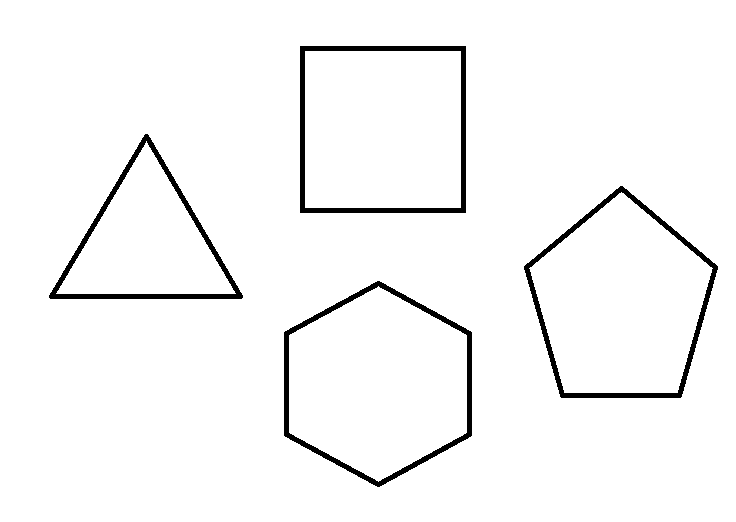
\includegraphics[width=0.5\textwidth]{polygon.png}
\end{figure}

\begin{center}
\Large $\sigma19.7$. Physics Medley\\
\end{center} \small
\mel{Barbie Girl}
I'm a physics boy, in a physics world.\\
Life in physics, it's all mathy\\
You can derivate, and sometimes integrate\\ 
Mathematics, it's your friend
\vspace{5pt}\\
Come on students let's go study!
\vspace{5pt}\\
We're all physics gals, in a physics world\\
We know about gas, a bit of light as well\\
in the end, its all energy
\nysida{15}{19.7}
\setlength{\oddsidemargin}{-0.37in}
\noindent
\mel{Wonderwall}
Today was gonna be the day\\
But I'll never understand at all\\
By now I should've somehow\\
Realized I'm never gonna do\\
I don't believe that anybody\\
Could do worse than I do, right now… 
\vspace{5pt}\\
And all the stuff to learn are complicated\\
And all the lights that lead me there are blinding\\
There are many things that I\\
Would like to learn right now,\\ 
but I don't know how
\vspace{5pt}\\
I said maybe,\\
you're gonna be the one to teach me\\
And after all,\\
you're my övningsassistent 
\vspace{5pt}\\
\mel{Blowin' in the wind}
How many tests must a student pass\\
Before you call him a physicist?\\
How many lectures must we attend\\
Before we leave forever? \\
The answer my friend is indeterminate\\
The answer is indeterminate 

\begin{flushright}
\textit{Harald Bjurulf, F-18 \\ Tentagasque 3: Mars \& Mello}
\end{flushright}

\nysida{15}{19.8}
\setlength{\oddsidemargin}{-0.47in}
\begin{center}


\Large $\sigma19.8$. Tjo va dé va livat i Kons \\
\mel{Tjo va dé va livat i holken}
\end{center} \small
Goder afton, får jag lov att presentera mig,\\
jag är fysiker och jag heter Filip\\
Är ni tillståndsenhet och vill studera mig\\
så passa på för nu är det så dags.\\
Jag har fått ett litet märke som ni nog kan se\\
i min övriga ovve någonstans.\\
Ja, det börja häromkvällen på en sektion breve,\\
där min Klubbis gav middag med dans.
\vspace{5pt}\\
Tjo vad de’ va’ livat i Kons där i fredags,\\
Christoffer, han fastna med väktaren i kläm.\\
Tjo vad de’ va’ livat i Kons där i fredags\\
uti de tokiga fysikernas hem.\\
Tjo vad de’ va’ livat i Kons där i fredags\\
alla for runt i en flygande dans.\\
Tjo vad de’ va’ livat i Kons där i fredags,\\
fulla i fan är vi lite till mans.
\vspace{5pt}\\
Shit, holy shit ropa Julia förskräckt,\\
Julia förskräckt, ja just Julia förskräckt.\\
Kom, alla pluggisar, (ingen är näck) \\
för nu är det promille direkt!
\vspace{5pt}\\
Tjo vad de’ va’ livat i Kons där i fredags\\
Grupprummet var fullt av dom som inte gick hem.\\
Tjo vad de’ va’ livat i Kons där i fredags\\
uti de tokiga fysikernas hem.
\newpage
\setlength{\oddsidemargin}{-0.37in}
\noindent
Jag tror alla vilda studenter som på campus fanns\\
ställde upp på vår nattliga zwyck,\\
Ja det var ju några wraque\\
som var för fulla för att få rum nånstans\\
Men till dem bar vi ut både föda och dryck.\\
Hela natten höll vi på med både stoj och glam,\\
stick i stäv mot vår pluggismoral\\
Så när solen sen på söndagsmorron titta fram\\
då var det lögn att få se en integral
\vspace{5pt}\\
Men, tjo vad de’ va’ livat i Kons där i fredags,\\
aldrig man skådat en muntrare gask.\\
Tjo vad de’ va’ livat i Kons där i fredags,\\
borta i ett hörn var det dragkamp om flask.\\
Tjo vad de’ va’ livat i Kons där i fredags,\\
Beta och Matlab syntes alls ingenstans.\\
Tjo vad de’ va’ livat i Kons där i fredags,\\
Plugget och fest var i bästa balans
\vspace{5pt}\\
Shit holy shit det var långt ifrån torrt\\
Långt ifrån torrt, ja just långt ifrån torrt\\
Sura i krävan vi vinglade bort\\
Men kommo tillbaks inom kort
\vspace{5pt}\\
Tjo vad de’ va’ livat i Kons där i fredags,\\
Linnea hon styrde i flygande fläng\\
Tjo vad de’ va’ livat i Kons där i fredags,\\
Uti de tokiga fysikernas hem.

\begin{flushright}
\textit{Filip af Malmborg, F-17 \\ Tentagasque 3: Mars \& Mello}
\end{flushright}

\nysida{15}{19.9}
\setlength{\oddsidemargin}{-0.47in}

\begin{center}
\Large $\sigma19.10$. En kväll i juli \\
\mel{En kväll i juli}
\end{center}\small Ja det va' en kväll i juli,\\
då när sommarn e' som bäst.\\
Det var skärgårdsfest på Husarö,\\
som en gillar allra mest.\\
Anders Borg han satt å nynna \\
på en sommarmelodi. \\
Plötsligt spratt de' till i gubben, \\
han blev full, för mycket vin...
\vspace{5pt}\\
Han tog av sig sin kavaj,\\ 
sparka av sig båda skorna \\ 
och sen drog han ner gylfen och sa\\
"Ska vi mäta våra kön?"\\
Han var full, som ett svin,\\ 
Anders Borg fick en "blackout"!\\
Sommarkvällen den var fin, \\
för Dominika var det pin
\vspace{5pt}\\
Na na na na na…. 
\vspace{5pt}\\
Ja det va' en morgon i juli,\\
då när sommarn e' som sämst.\\
Folk hade huvudvärk på Husarö\\
och då Anders allra främst.\\
Anders han hade sumpat \\
sitt uppdrag på Kinnevik.\\
Festen blev ej som han tänkt sig,\\
vardagen sig aldrig lik.
\newpage
\setlength{\oddsidemargin}{-0.37in}
\noindent
Om du är på skärgårdsfest,\\
varannan vatten kan va bäst.\\
Vi vill säga med denna sång, \\
att det finns gränser för hålligång!\\ 
Lyssna noga, på oss,\\
lär dig den här läxan: \\
om du ej vill känna sorg\\
lär dig då av Anders Borg!\\

\begin{flushright}
\textit{Jakob Stymne, F-17\\ Tentagasque 4: Skandal!}
\end{flushright}

\nysida{15}{19.10}
\setlength{\oddsidemargin}{-0.47in}
\begin{center}
\Large $\sigma19.10$. Fysikmedley
\end{center}\small 
\mel{Gammal sång}
Friläggning, friläggning i min kalender idag,\\
ingen frihet kvar.\\
Tjugosex, tjugosex variabler till hands,\\
vill flytta utomlands.
\vspace{5pt}\\
Stackars mig, fick bara 5 minuters rast idag!\\
Vill inte höra någon säga mig, \\
det här är uppenbart, det ser ni snart...
\vspace{5pt}\\
Till alla er som känner er lite vilsna,\\
såhär innan lovet
\vspace{5pt}\\
\mel{One}
Har ni kommit för betygen,\\ 
har ni kommit för er självbild,\\
har ni kommit för verktygen, \\
att kunna skicka mail till pär, då ska jag \\
berätta, leta ej här, för ni vet redan vem ni är 
\vspace{5pt}\\
\mel{Måndagsbarn}
Jag var ett jobbigt barn, inte bara massa gnäll\\
Jag ville veta allt, ingen tyckte jag var snäll
\vspace{5pt}\\
Så en lördag klockan 5,\\ 
nån nämnde nått var jag skulle, hitta hem,\\
för stunden, var jag nöjd men, bara män, \\
har fått nog fysik
\vspace{5pt}\\
\mel{Killing me softly}
Kanske behöver vi blunda, famla och ha lite fel,\\
kanske behöver vi strunta, i alla våra besvär,\\
Gå matte och bli miljardär!
\begin{flushright}
\textit{Julia Schauman, F-17 \\ Tentagasque 4: Skandal!}
\end{flushright}
\nysida{15}{19.11}
\setlength{\oddsidemargin}{-0.37in}
\noindent
\begin{center}
\LARGE Fysikalen \\
\end{center}
\begin{center}
\Large $\sigma19.11$. Fysikalenmåsen \\
\mel{Månvisa}
\end{center}\small
\vspace{30pt} \textbf{A-skådismås (Påfågel)}
\vspace{5pt}\\
Det satt en skådis ut i en loge,\\
en riktig diva var kräket\\
Allt skall serveras i silverskål\\
Så man får tyst på mjäket\\
Regin den rope: “Sluta va svår!”,\\
och skådis svarte: “Showen är vår!\\
Störst skådis är. Så släng det här!”
\vspace{30pt}\\
\textbf{Kör-mås (Sångfågel)}
\vspace{5pt}\\
Det stod en kör nånstans bakom scen\\ 
Och de sjöng där i sin stämma\\
Deras repliker har tagits bort\\
Det här kan ju inte stämma\\
“Vi vill va me” hördes kören sjunge\\
De kändes små som en ankunge\\
Men dess noter var, de flesta kvar
\newpage
\setlength{\oddsidemargin}{-0.47in}
\noindent
\vspace{30pt}\\
\textbf{Dekor-mås (Svala)}
\vspace{5pt}\\
Dekoren har byggt allting på scen\\
De både kämpar och sliter\\
Med gångjärnsdörrar och trix å fix\\
Vänta! Ett misstag begicks\\
Och de ser nu till sin förtvivlan\\
Att slottsporten är inte helt grann\\
Den är ej hel, Hedengrens fel
\vspace{30pt}\\
\textbf{Bromsmås (Nötväcka)}
\vspace{5pt}\\
Det satt en spökmås ut på en kvist\\
Han hette Henrik med åtta\\
Han orarerar men ingen hör\\
Nu ska han feta rhymes spotta\\
MEN\\
När han ska sjunga och få all äran\\
Inser han nu till sin förfäran\\
Han glömde å slå myggan på

\begin{flushright}
\textit{Philip Broms, F-15 \\ Fysikalens Slutfest 2018}
\end{flushright}
\newpage
\nysida{15}{19.12}
\setlength{\oddsidemargin}{-0.37in}

\begin{center}
\Large $\sigma19.12$. En gaffa kort \\
\mel{En gaffel kort}
\end{center} \small 
Ville skydda våra öron, sätta trummis i en bur. \\
Och resten av orkestern döljs helt utav en mur. \\
Men fullt så höga murar blev det inte på vårt fort. \\
Fick nöja oss med hälften för vi var en gaffa kort.
\vspace{5pt}\\
En gaffa kort, en gaffa kort.\\
Orkestern syns och hörs för att vi var en gaffa kort.
\vspace{5pt}\\
Kulisserna ska resas, ljusläckor tätas till\\
Då duger inte tvingar, de gör inte som man vill\\
Och vi lyckas inte täta vårat jättesnygga slott\\
Normalt hade det gått, men nu var vi en gaffa kort
\vspace{5pt}\\
Första akten den har börjat, andra numret är förbi\\
I mörkret bakom scenen i en vrå där sitter vi\\
Försöker laga det som Gustav pajat som en sport\\
Det hade varit lätt om man ej var en gaffa kort.
\vspace{5pt}\\
En gaffa kort, en gaffa kort.\\
Kan laga vad som helst om man ej är en gaffa kort.
\vspace{5pt}\\
Akt 2 den börjar nu och har en bar av högsta klass\\
Men under baren är det mörkt och sikten den är kass.\\
På golvet har en tejpmarkeringsbana tappats bort\\
Att köra baren rakt är svårt\\
när man är en gaffa kort
\vspace{5pt}\\
Ridån går upp en tredje gång med Hedengren på scen\\
Han lutar sig mot en kuliss som verkar ganska klen.\\
Kulissen som fixeras med ett fäste av nån sort\\
Men inte denna dagen för vi var en gaffa kort.
\vspace{5pt}\\
En gaffa kort, en gaffa kort.\\
Kulissen vore hel ifall vi var en Gustav kort.
\nysida{15}{19.13}
\setlength{\oddsidemargin}{-0.47in}
\noindent
Vårt spex det är nu färdigt, publiken har gått ut.\\
Och framför scenens blanka golv\\
det plötsligt hörs ett tjut\\
Där står tekniken krossade och gråter lite smått\\
För nu har även nyinköpta gaffan tappats bort,\\
Hur säkrar vi kulisserna i lastbil för transport?\\
Vår vas den gick i kras för att vi var en gaffa kort.
\vspace{5pt}\\
Vad ska nu denna visa ha för sensmoral?\\
Jo om du nån gång blir bjuden att gå med i en fysikal\\
Se då till att göra audition\\
För en scengrupp av nån sort\\
då spelar det ingen roll ifall du är en gaffa kort

\begin{flushright}
\textit{Teknikgruppen \\ Fysikalens Slutfest 2018}
\end{flushright}
\begin{center}
\LARGE Övrigt \\
\end{center}
\begin{center}
\Large $\sigma19.13$. Systéme Fruktinationale\\
\mel{Studentsången}
\end{center} \small 
ananas apelsin aprikos\\
banan carambola citron citrusfrukt\\
clementin carambola \\
granatäpple grapefrukt\\
kaktusfikon kumquat kiwi lime\\
mandarin mango melon nektarin\\
papaya passionsfrukt persika\\
plommon päron satsuma\\
plommon päron satsuma sharon!
\begin{flushright}
\textit{Text: https://sv.wikipedia.org/wiki/Frukt\#Frukter\\ Framförd av Hanna Kylhammar, F-17 \\ Open-gasquen 2018}
\end{flushright}
\nysida{15}{19.14}
\setlength{\oddsidemargin}{-0.37in}
\begin{center}
\Large $\sigma19.14$. Plan i grus\\
\mel{Stad i ljus}
\end{center} \small Min resa var mot solen,\\
långt bort från alla mötesrum.\\
Där brunchen är oändlig,\\
min första charter kommer aldrig att ta slut.
\vspace{5pt}\\
Jag ville se miraklet,\\
och höra skrik från nyfött liv.\\
Bli buren av en styrka,\\
och visiteras för de tror att jag har kniv.
\vspace{5pt}\\
Plan i grus, i ett land utan namn.\\
Ge mig vin, svindyra snacks är värt.
\vspace{5pt}\\
Och så när allt förändrats,\\
när vingar inte längre finns.\\
Så ser jag oss tillsammans\\
och då är resan slut, det enda som vi minns.
\vspace{5pt}\\
$\|$: Plan i hus, i ett land utan namn.\\
Rädda ditt liv, innan du räddar den bredvid. :$\|$

\begin{flushright}
\textit{Helmer Nylén, F-15, och Hanna Kylhammar, F-17\\ Mottagningens Vårfest 2019}
\end{flushright}

\end{document}